\section{Background}
\label{sec:background}

\vspace{5pt}
\noindent \uline{Historical work.}
Very early work on improving cluster memory 
utilization ~\cite{gms,cashmere,treadmarks,dsm1} 
sticked to traditional server architectures and focused on 
software-based memory pooling across the cluster and exposing it 
to applications in (mainly) two different flavors. 
Distributed shared memory (DSM) systems~\cite{treadmarks,dsm1} 
provide a global shared address space for writing distributed 
applications, where the address space is globally accessible 
from all the servers. These systems can then transparently 
back subsets of address space (at different granularity) with 
physical memory from different servers across the cluster, and 
therefore have the flexibility of optimizing cluster memory 
utilization. Other systems like GMS~\cite{gms, cashmere} just 
focus on extending the address space of individual applications 
without any notion of sharing across servers (i.e., their memory 
consistency model stops with cache coherence protocols on a single 
server). These systems merely back or complement local DRAM with 
unutilized memory from other servers using the paging mechanisms 
in the operating system, usually by providing remote memory as 
another block device to swap to. DSM systems 
provide shared memory (along with some consistency model) which 
makes distributed programming easier but they may require 
applications be rewritten using their memory model. Conversely, 
remote paging systems aim to be more backwards-compatible and 
leave the complexity of building distributed applications 
(if needed) to the higher layers. These early systems however 
hasn't seen adoption (perhaps?) because remote memory latencies 
were still far higher for tenable application performance. 
(DSM though had even more challenges due to overheads in 
ensuring consistency that get amplified with slow networks).

\vspace{5pt}
\noindent \uline{Recent proliferation in this space.}
With the advent of faster networks and technologies such as 
RDMA~\cite{farm} to commodity clusters, there has been a renewed 
interest in building such systems. 
As remote access latencies 
get closer to native DRAM latencies (which, on the contrary, 
are nearing saturation~\cite{Aguilera2017}),
writing applications with such accesses 
in the critical path is looking feasible, 
performance-wise~\cite{netdisagg}. 
Consequently, there has been a lot of RDMA-inspired remote 
memory system building in recent years, including a renewal in
DSM~\cite{farm, gam,dspm,ltdsm} and Remote 
paging~\cite{Lim2012,bladedisagg1,infiniswap,zswap,fastswap,leap} 
systems. While the remote paging systems provide native virtual memory 
interface (i.e., memory access through load/store ops on cached 
local pages from remote memory) to applications, 
other new interfaces for remote memory were proposed that 
sacrifice application transparency in favor of performance 
due to either the simplicity of 
implementation~\cite{remregions,literdma} (light-weight runtime 
means less performance overhead in the critical access path) or 
benefits from application hints~\cite{aifm}; 
conversely, these interfaces require app modifications but
enable applications to distinguish between local and remote 
memory accesses and be smart about it e.g., use far-memory 
aware implementations~\cite{Aguilera2019,semeru}.

Most systems for disaggregated memory target clusters with 
traditional (commodity) servers where memory is collocated 
with processors and there is no special hardware support.
Traditional hardware cannot access remote memory directly 
 and hence usual solutions has to proxy it  
through local memory by caching remote data and resorting to 
software to fetch remote data on a cache miss. To avoid 
this overhead, some systems introduce special hardware 
like a remote memory controller~\cite{sonuma} or a 
cache-coherent FPGA~\cite{kona} to plug into 
the local cache hierarchy and handle remote accesses through 
the hardware. And finally, as an alternative to traditional 
server model, there were proposals for new 
hardware architectures where memory is decoupled and pooled
at a hardware-level, and some systems targeting such 
disaggregation~\cite{sonuma,bladedisagg1,legoos} as well, 
a note-worthy one of which is LegoOS~\cite{legoos}. In this 
report, we will look at many of these systems to provide an 
informed view of disaggregated system design.

\begin{figure*}[h!]
\centering
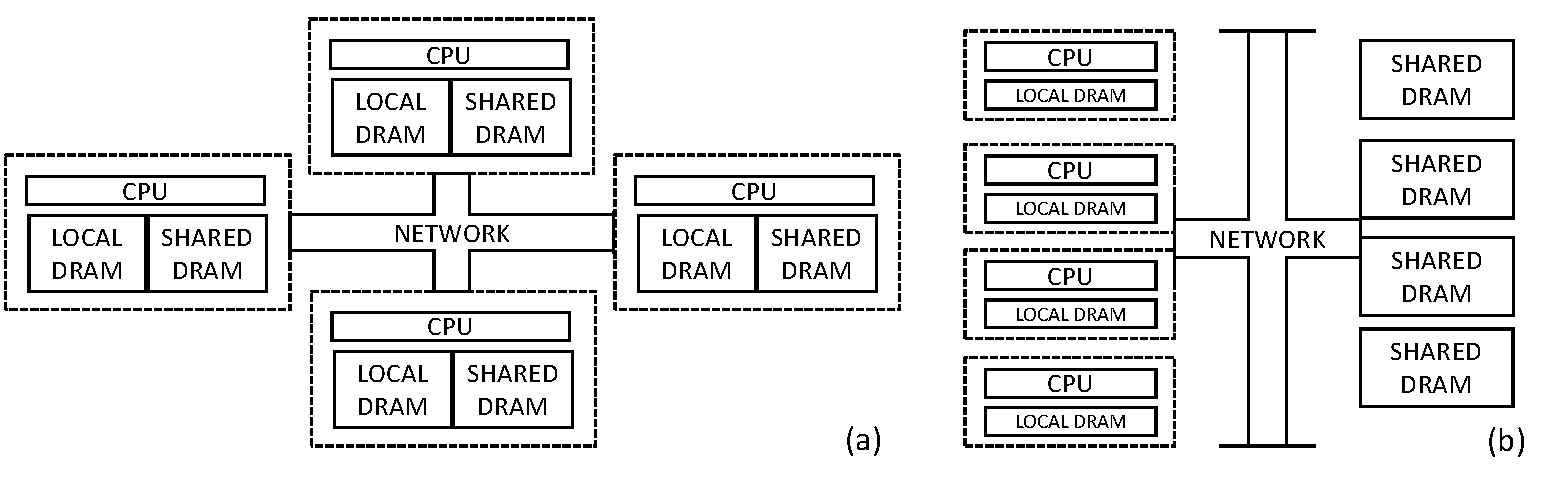
\includegraphics[width=.9\linewidth]{fig/architecture.pdf}
\caption{(too big?) Shows (a) software-disaggregated architecture where disaggregated memory is pooled from 
traditional servers as opposed to the (b) hardware-disaggregated
design where most memory is decoupled in hardware.}
\label{fig:architecture}
\end{figure*}